%! Author = albert
%! Date = 11.04.2021

% Preamble
\documentclass[11pt]{article}

% Packages
\usepackage[T1]{fontenc}
\usepackage[utf8]{inputenc}
\usepackage{latexsym,amsmath,amssymb,amsthm}
\usepackage{multicol}
\usepackage{graphicx}
\usepackage{geometry}
\usepackage{lipsum}
\usepackage{breqn}
\usepackage{longtable}
\usepackage{enumerate}
\usepackage{subfig}
\usepackage{subfigure}
\usepackage{linegoal}
\usepackage{graphics}
\usepackage{tabularx}
\usepackage{pdflscape}
\usepackage{bm}
\usepackage{empheq}
\usepackage{url}
\usepackage{adjustbox} %dopasowanie tabeli
\usepackage{float} % zmuszanie obrazków do bycia w konkretnym miejscu
\usepackage{floatrow} % kilka obrazków w lini dla float

\usepackage{listings}
\lstset{escapeinside={<@}{@>}}


\renewcommand{\arraystretch}{1,25}

\title{Big Data Analytics\\ Statistical Physics\\ 2D Ising model}
\author{Albert Piekielny 244951\\}
\date{30.05.2021}


%% Uncomment to change margins size
\geometry{top=2.5cm,bottom=2cm,left=2.5cm,right=2.5cm}

\DeclareMathOperator{\sgn}{sgn}
\newcommand{\mA}{\bm{A}}
\newcommand{\mB}{\bm{B}}
\newcommand{\mC}{\bm{C}}
\newcommand{\mL}{\bm{L}}
\newcommand{\mU}{\bm{U}}
\newcommand{\mZ}{\bm{0}}
\newcommand{\vb}{\bm{b}}
\newcommand{\vx}{\bm{x}}
\newcommand{\R}{\mathbb{R}}


% Document
\begin{document}
    \maketitle


    \section{Introduction}
    \label{sec:introduction}


    The main simulation program was written in Java version 15.\ The plots were generated using the plotly library in Python.
    The simulation was based on the analysis of the average value of the system energy as well as the magnetization for $K = 230 000$.
    For this purpose, mean values ranging from $K0 = 30 000$ were calculated every $100$ iterations of the main loop.
    For each of the simulations, the change in the coefficient $T^*$ was $\Delta t=0.01$.


    \section{Presentation results}
    \label{sec:results}

    \subsection{Exemplary configurations of spins}
    \label{subsec:exemplary-configurations-of-spins}

    \begin{figure}[H]
        \centering
        \subfigure[]{
            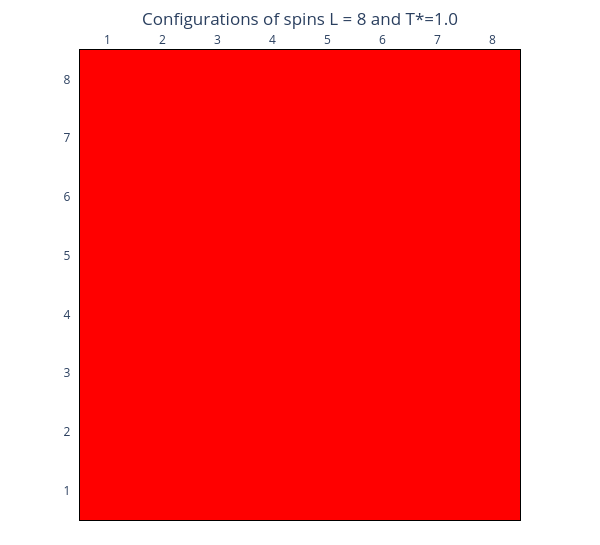
\includegraphics[width=0.31\linewidth]{img/spins_L8_T1.0}
        }
        \subfigure[]{
            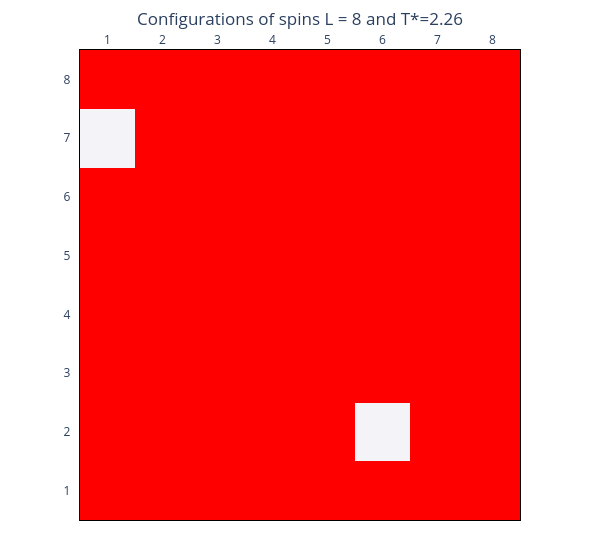
\includegraphics[width=0.31\linewidth]{img/spins_L8_T2.26}
        }
        \subfigure[]{
            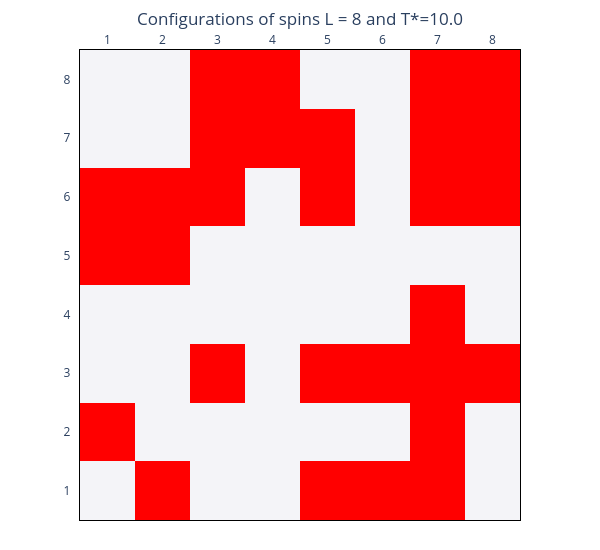
\includegraphics[width=0.31\linewidth]{img/spins_L8_T10.0}
        }
        \caption{Example spin configurations for $L = 8$ and $T* = 1.0$,\ $T* = 2.26$,\ and $T* = 10$ }
        \label{fig:first}
    \end{figure}

    \begin{figure}[H]
        \centering
        \subfigure[]{
            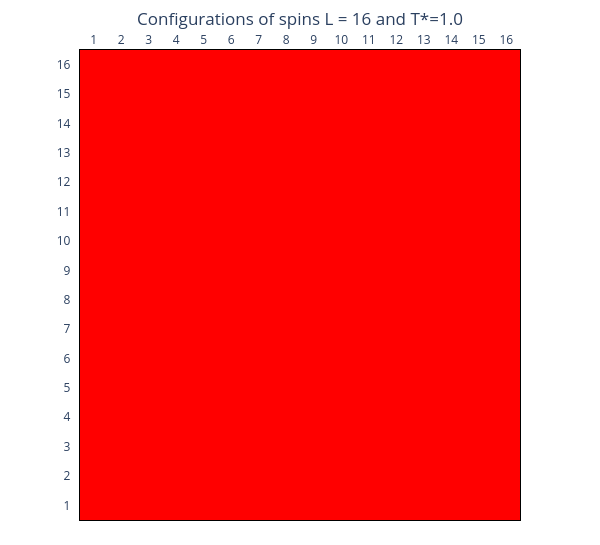
\includegraphics[width=0.31\linewidth]{img/spins_L16_T1.0}
        }
        \subfigure[]{
            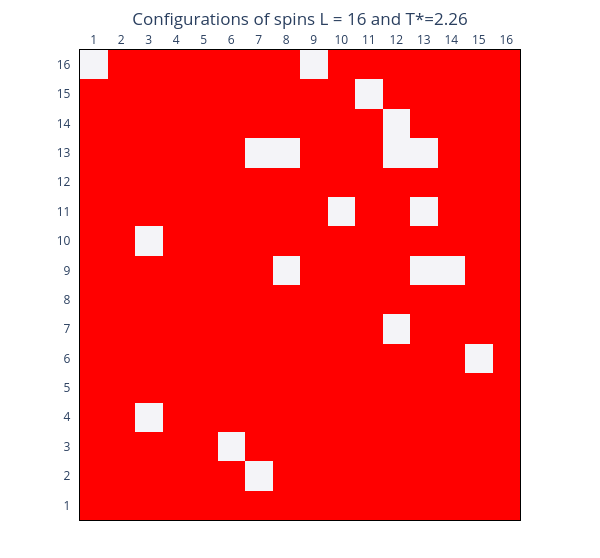
\includegraphics[width=0.31\linewidth]{img/spins_L16_T2.26}
        }
        \subfigure[]{
            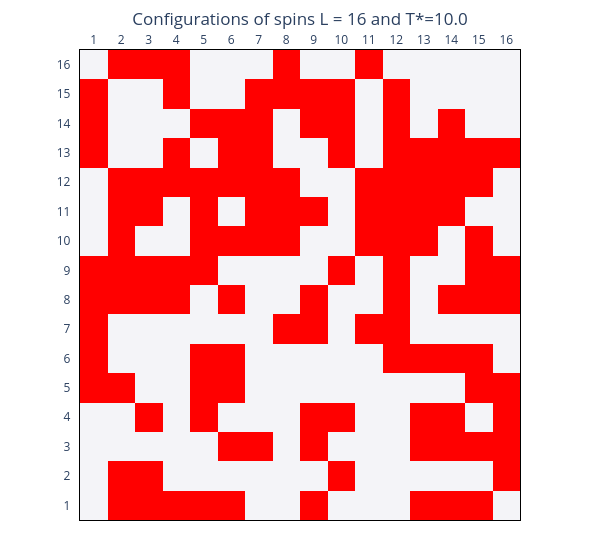
\includegraphics[width=0.31\linewidth]{img/spins_L16_T10.0}
        }
        \caption{Example spin configurations for $L = 16$ and $T* = 1.0$,\ $T* = 2.26$,\ and $T* = 10$ }
        \label{fig:second}
    \end{figure}

    \begin{figure}[H]
        \centering
        \subfigure[]{
            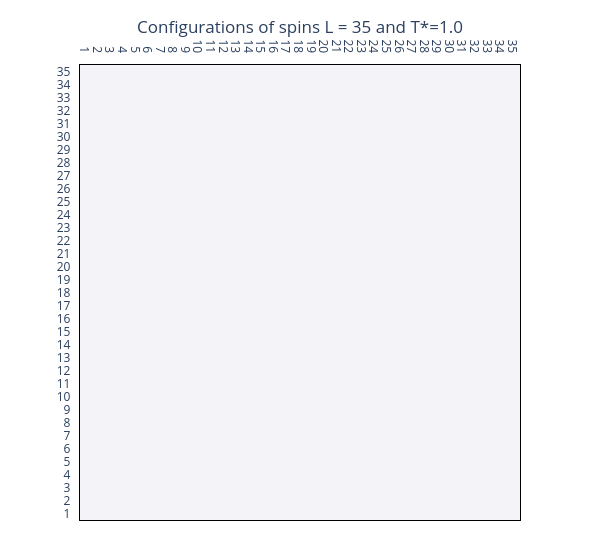
\includegraphics[width=0.31\linewidth]{img/spins_L35_T1.0}
        }
        \subfigure[]{
            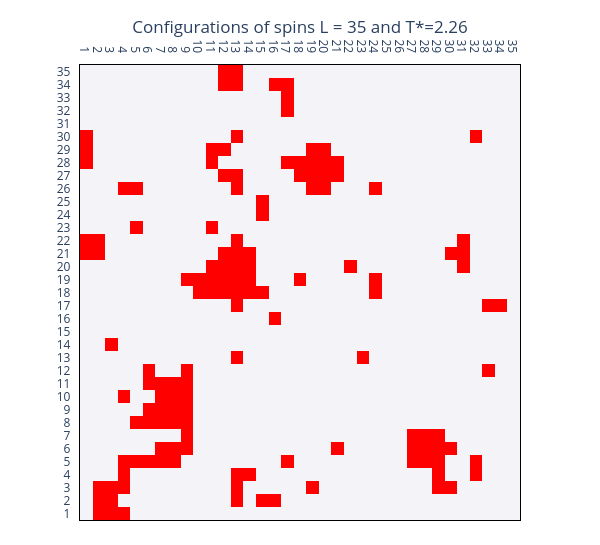
\includegraphics[width=0.31\linewidth]{img/spins_L35_T2.26}
        }
        \subfigure[]{
            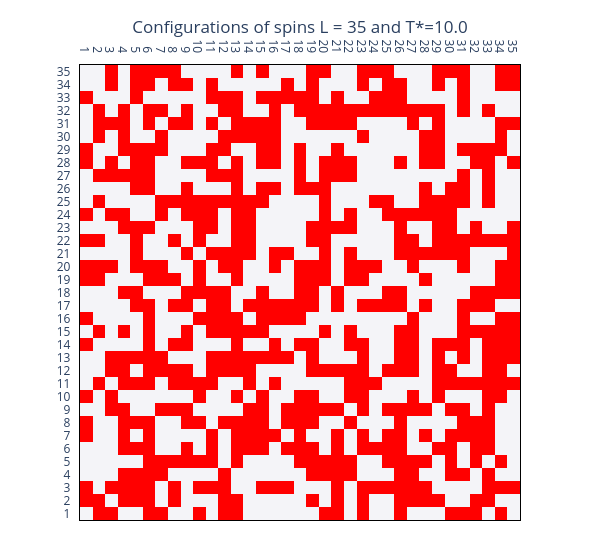
\includegraphics[width=0.31\linewidth]{img/spins_L35_T10.0}
        }
        \caption{Example spin configurations for $L = 35$ and $T* = 1.0$,\ $T* = 2.26$,\ and $T* = 10$ }
        \label{fig:tird}
    \end{figure}


    \subsection{Average values}
    \label{subsec:average-values}

    The results for magnetization and heat capacity were averaged after $230 000$ Monte Carlo
    steps.\ Each 100-th configuration was analyzed after first $30 000$ steps.\ Temperatures $T^*$
    that were used as parameters are as follows $1.5, 1.51, 1.52, \ldots, 3.50$.

    \begin{figure}[H]
        \centering
        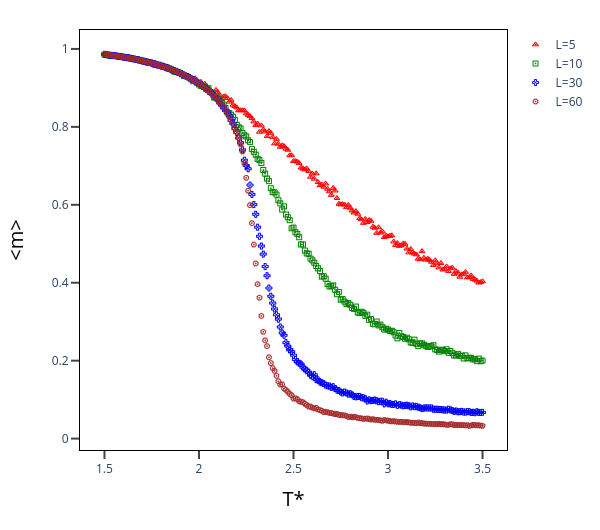
\includegraphics[width=0.75\linewidth]{img/magnetisation}
        \caption{: Magnetization against temperature T}
        \label{fig:fourth}
    \end{figure}

    \begin{figure}[H]
        \centering
        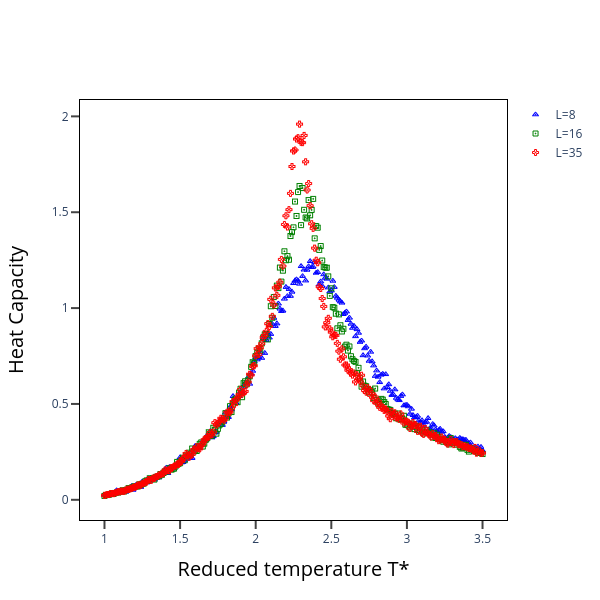
\includegraphics[width=0.75\linewidth]{img/heat}
        \caption{: Heat Capacity against temperature T}
        \label{fig:fifth}
    \end{figure}


    \section{Source code}
    \label{sec:code}

    \newgeometry{left=5mm, right=10mm, top=1.5cm, bottom=1cm}
    \begin{small}
        \begin{lstlisting}[language=Java, frame=lines, numberstyle=\tiny, stepnumber=5,
            caption=Java Simulation Code \label{hibernate-properties}., firstnumber=1,label={lst:code}]
import java.io.FileWriter;
import java.io.IOException;
import java.util.Random;
import java.util.function.Function;
import java.util.stream.IntStream;

public class IsingModel2D {

    private static final Random rand = new Random(System.nanoTime());
    private static final String outMagnetisationFilePattern = "magnetization_file_L%d.txt";
    private static final String outHeatFilePattern = "heat_file_L%d.txt";
    private static final int MCS = 230_000;
    private static final int K0 = 30_000;

    private record Pair(double val1, double val2) {
    }

    public static void main(String[] args) {
        final IsingModel2D isingModel2D = new IsingModel2D();
        isingModel2D.avgHeatSimulation();
        isingModel2D.avgMagnetisationSimulation();
        isingModel2D.exampleSpinConfiguration();

    }

    public void avgMagnetisationSimulation() {
        int[] latticeSizeDef = {5, 10, 30,60};
        for (int l : latticeSizeDef)
            twoDimIsingModelSimulation(l, 1.5, 3.5, 0.01, outMagnetisationFilePattern, Pair::val1);
    }

    public void avgHeatSimulation() {
        int[] latticeSizeDef = {8, 16, 35};
        for (int l : latticeSizeDef)
            twoDimIsingModelSimulation(l, 1.0, 3.5, 0.01, outHeatFilePattern, Pair::val2);
    }

    private void periodicBoundaryConditionStep(int i, int j, int[][] matrix, double tStar) {
        int delta_energy = 2 * (matrix[i][j]) * getNeighborSum(i, j, matrix);
        if (delta_energy < 0 || rand.nextDouble() <= Math.exp(-delta_energy / tStar))
            matrix[i][j] = -matrix[i][j];
    }

    private int getNeighborSum(int i, int j, int[][] matrix) {
        int matrixSize = matrix.length;
        int up = (i == 0) ? matrix[matrixSize - 1][j] : matrix[i - 1][j];
        int down = (i == matrixSize - 1) ? matrix[0][j] : matrix[i + 1][j];
        int left = (j == 0) ? matrix[i][matrixSize - 1] : matrix[i][j - 1];
        int right = (j == matrixSize - 1) ? matrix[i][0] : matrix[i][j + 1];
        return (left + right + up + down);
    }

    private int[][] generateSquareMatrix(int size) {
        int[][] matrix = new int[size][size];
        IntStream.range(0, size)
                .forEach(i -> IntStream.range(0, size)
                        .forEach(j -> matrix[i][j] = rand.nextDouble() > 0.5 ? 1 : -1));
        return matrix;
    }


    private Pair MSCStep(int[][] matrix, double tStar) {
        int matrixSize = matrix.length;
        double avm = 0.0, avEnergy = 0.0, av2Energy = 0.0;
        double avgSteps = (MCS - K0) / 100.0;
        for (int k = 1; k <= MCS; k++) {
            for (int i = 0; i < matrixSize; i++)
                for (int j = 0; j < matrixSize; j++)
                    periodicBoundaryConditionStep(i, j, matrix, tStar);

            if (k > K0 && k % 100 == 0) {
                avm = avm + Math.abs(calculateMagnetisation(matrix, matrixSize));
                double energy = calculateEnergy(matrix, matrixSize);
                avEnergy += energy;
                av2Energy += (energy * energy);
            }
        }
        avm = avm / avgSteps;
        avEnergy /= avgSteps;
        av2Energy /= avgSteps;
        double heat = 1.0 / (matrixSize * matrixSize * tStar * tStar)
                            * (av2Energy - (avEnergy * avEnergy));
        return new Pair(avm, heat);
    }

    private double calculateMagnetisation(int[][] matrix, int matrixSize) {
        double m = 0;  //magnetisation
        for (int[] ints : matrix)
            for (int j = 0; j < matrixSize; j++)
                m += ints[j];
        m = m / (matrixSize * matrixSize);
        return m;
    }

    private int calculateEnergy(int[][] matrix, int matrixSize) {
        int energy = 0;
        for (int i = 0; i < matrixSize; i++)
            for (int j = 0; j < matrixSize; j++)
                energy += (matrix[i][j] * getNeighborSum(i, j, matrix));
        return energy / 2;
    }


    private void twoDimIsingModelSimulation(int lattice_size, double t0, double t_end,
                                            double step,
                                            String outFilePattern,
                                            Function<Pair, Double> func) {
        t_end += 9.0E-13;
        try (var writer = new FileWriter(String.format(outFilePattern, lattice_size))) {
            for (double tStar = t0; tStar < t_end; tStar += step)
                Pair data = MSCStep(generateSquareMatrix(lattice_size), tStar);
                writer.write(tStar + " " + func.apply(data) + "\n");
        } catch (IOException e) {
            e.printStackTrace();
        }
    }

        public void exampleSpinConfiguration(){
        int[] latticeSizes = {8, 16, 35};
        double[] tStars= {1.0, 2.26, 10.0};
        for (int lSize : latticeSizes) {
            for (double tStar : tStars) {
                final int[][] matrix = generateSquareMatrix(lSize);
                for (int k = 1; k <=MCS ; k++) {
                    for (int i = 0; i <lSize; i++)
                        for (int j = 0; j < lSize; j++)
                            periodicBoundaryConditionStep(i,j,matrix,tStar);
                }
                saveContent(matrix, String.format("config_L=%d_T=%f.txt", lSize, tStar));
            }
        }
    }

    private static void saveContent(int[][] model, String outFilePattern) {
        final StringBuilder sb = new StringBuilder();
        for (int[] ints : model)
            sb.append(String.join(" ",
                    IntStream.of(ints)
                            .mapToObj(s -> "" + s)
                            .toArray(String[]::new))).append('\n');
        writeStringToFile(outFilePattern, sb.toString());
    }

    private static void writeStringToFile(final String outPath, final String content) {
        try (var fileWriter = new FileWriter(outPath)) {
            fileWriter.write(content);
        } catch (IOException e) {
            e.printStackTrace();
        }
    }
}

        \end{lstlisting}
    \end{small}

    \begin{small}
        \begin{lstlisting}[language=Python, frame=lines, numberstyle=\tiny, stepnumber=5,
            caption=Python Plots Code \label{python-plots}., firstnumber=1,label={lst:code2}]
from typing import List

import plotly.graph_objects as go


def heatmap_chart(matrix: List[List[int]], L, t_star) -> None:
    import plotly.figure_factory as ff
    txt = [["" for _ in range(len(matrix))] for _ in range(len(matrix))]
    labels = [i + 1 for i in range(len(matrix))]
    tmp = []
    for i in range(len(matrix) - 1, -1, -1):
        tmp.append(matrix[i])
    fig = ff.create_annotated_heatmap(tmp, annotation_text=txt,
                                      colorscale=['rgb(244,244,248)', 'rgb(255,0,0)'],
                                      zmin=-1, zmax=1, showscale=False, x=labels, y=labels[::-1])
    fig.update_xaxes(showline=True, linewidth=1, linecolor='black', mirror=True)
    fig.update_yaxes(showline=True, linewidth=1, linecolor='black', mirror=True)
    fig.update_layout(width=600, height=600,
                      title=f'Configurations of spins L = {L} and T*={t_star}', margin_t=65,
                      title_x=0.5,
                      legend_title_side='top')
    fig.show()


def point_plot(scatter: list, x_title, ytitle) -> None:
    fig = go.Figure()
    for s in scatter:
        fig.add_trace(s)
    fig.update_layout({'plot_bgcolor': 'rgb(255, 255, 255)', 'paper_bgcolor': 'rgb(255, 255, 255)'},
                      width=600, height=600)
    fig.update_xaxes(showline=True, linewidth=1, linecolor='black', mirror=True, ticks='outside',
                     tickwidth=2, ticklen=8, title=x_title, title_font_size=20,
                     title_font_color='black')
    fig.update_yaxes(showline=True, linewidth=1, linecolor='black', mirror=True, ticks='outside',
                     tickwidth=2, ticklen=8, title=ytitle, title_font_size=20,
                     title_font_color='black')
    fig.show()


def create_scatter_plot(l_defs: List[str], filename: str) -> List:
    scaters = []
    markers = ['triangle-up-open-dot', 'square-open-dot',
               'cross-open-dot', 'octagon-open-dot', 'triangle-up-open-dot']
    colors = ['blue', 'green', 'red', 'brown']
    counter = 0
    for l in l_defs:
        with open(filename.format(l), 'r') as open_file:
            x = []
            y = []
            for line in open_file.readlines():
                split = line.split()
                x.append(float(split[0]))
                y.append(float(split[1]))
            df = dict({'x': x, 'y': y, })
            scaters.append(go.Scatter(df, x=x, y=y, mode='markers', name=f"L={l}",
                                      marker=dict(size=5, color=colors[counter],
                                                  symbol=markers[counter])))
            counter += 1
    return scaters


def read_matrix(filNam: str):
    matrix_list = []
    with open(filNam, 'r') as matrixFile:
        for line in matrixFile.readlines():
            line = line.split()
            line = [int(i) for i in line]
            matrix_list.append(line)
    return matrix_list


def example_spin_config():
    for l_size in [8, 16, 35]:
        for t_star in [1.0, 2.26, 10]:
            heatmap_chart(read_matrix(f"config_L={l_size}_T={t_star}.txt"), l_size, t_star)


if __name__ == '__main__':
    example_spin_config()
    point_plot(create_scatter_plot(['8', '16', '36'], "heat_file_L{l}.txt"),
               'Reduced Temperature T*', 'Heat Capacity')
    point_plot(create_scatter_plot(['5', '10', '30', '60'], "magnetization_file_L{l}.txt"),
               'T*', '<m>')

        \end{lstlisting}
    \end{small}

    \restoregeometry


\end{document}